\documentclass[10pt,twocolumn]{article}
\usepackage[colorlinks=true,linkcolor=black,urlcolor=black,citecolor=black]%
{hyperref}
\usepackage{graphicx}

\renewcommand{\t}{\texttt}

\title{Address space content randomization: \\
exploit mitigation through data randomization}
\author{Carlo Angiuli}

\begin{document}
\maketitle

\section{Introduction}

Address space layout randomization \cite{PaX} is a popular technique for
mitigating buffer overflow vulnerabilities in software. By randomizing the
memory layout of software when it is loaded into memory, and additionally
prohibiting memory pages from being both writable and executable, an attacker is
limited to guessing the address of any already-loaded code his or her exploit
executes.

However, these security mechanisms do not affect the layout of data on the
stack, permitting an attacker to access return pointers, and therefore, quickly
guess the memory offset of \t{libc} \cite{ShachamEtAl}. 

Notice that this attack is possible only because memory \emph{content} often
contains memory \emph{addresses}, thus leaking information about the randomized
layout. Furthermore, we observe that \emph{memory} is susceptible to replay
attacks, because it maps addresses to content in a deterministic fashion
\cite{Eckhardt}.

We propose a novel method for mitigating memory-related program exploits by
randomizing the \emph{content} stored at addresses in memory, which we call
Address Space Content Randomization (ASCR). This provides many benefits over
previous vulnerability mitigations:
\begin{enumerate}
\item By randomizing the contents of memory, we supercede the need to randomize
memory addresses via ASLR.
\item Our technique can be implemented in a per-application fashion, rather than
relying on kernel facilities.
\item Applications which run under ASCR are necessarily more robust, because
they cannot exploit memory replay attacks by expecting deterministic memory
behavior.
\item We drastically improve the performance of most applications by removing
the need to access memory.
\end{enumerate}

\section{Implementation}

We discuss our implementations of static and dynamic ASCR as LLVM optimization
passes, and the security and performance tradeoffs between these
implementations.

\subsection{Static ASCR}

In static ASCR, all memory reads are replaced by random numbers generated at
compile time. As a result, attackers who only have access to a program's source
code cannot craft successful exploits, as they cannot determine what behavior
the program will have when compiled.

As with ASLR, programmers must ensure that their software works correctly in the
presence of ASCR. In this case, local variables cannot be assumed to hold any
particular value, although they are guaranteed to hold the same value across
multiple invocations of a program. These strict guidelines promote a healthy
feeling of mistrust toward one's compiler, which in turn, promotes more robust,
secure software.

It is worth noting that ASCR requires no kernel support, unlike ASLR, and thus
can be adopted immediately---any programmer can immediately begin shipping code
which takes advantage of our strong security guarantees.

We have implemented an LLVM optimization pass which performs static ASCR
conversion on any LLVM bitcode, through the following transformations:
\begin{enumerate}
\item Load instructions are robustly replaced by random numbers.
\item Store instructions are removed, as they leak information.
\end{enumerate}
By following this by standard compiler optimizations, we achieve surprisingly
large speedups and code size reductions in a variety of benchmarks.

\subsection{Dynamic ASCR}

In dynamic ASCR, all memory reads are replaced by random numbers generated at
runtime. As a result, even attackers who have access to a program's binary
cannot craft successful exploits, as runtime behavior is unpredictable.

We use \t{libc}'s \t{rand} function to generate random numbers, reseeding it
with the time at the start of every program. This eases debugging, as
programmers can reproduce bugs by resetting their system clock each time they
run software with dynamic ASCR.

Dynamic ASCR relies only on the presence of a random number generator, and can
again be implemented without additional kernel support. Our LLVM optimization
pass is similar to the static ASCR pass:
\begin{enumerate}
\item Load instructions are robustly replaced by calls to \t{rand}.
\item Store instructions are removed, as they leak information.
\end{enumerate}
We achieve greater security than static ASCR, but at the cost of
performance---the dynamic nature of this feature reduces the optimization
opportunities available afterwards.

\section{Evaluation}

Our present implementations of ASCR randomize only data, but we anticipate
extending it to randomize code as well. This generalized form of ASCR entirely
supercedes the need for ASLR; while ASLR makes it difficult for attackers to
obtain pointers to protected regions of memory, ASCR simply decouples those
pointers from access to any program code or data.

Our observation is that all memory-related attacks hinge upon the association of
pointers with data in memory, so by stopping this attack vector entirely, we
secure software against a very large class of vulnerabilities.

\subsection{Performance}

As a simple integer benchmark, we implemented the industry-standard
recursive algorithm \cite{Angiuli,Angiuli} for Fibonacci numbers:
\begin{verbatim}
int fib(int x) {
  if (x == 0)
    return 1;
  else if (x == 1)
    return 1;
  else
    return fib(x-1) + fib(x-2);
}
\end{verbatim}
and computed \t{fib(50)}. We compiled the same \t{fib} function three ways: with
static ASCR (followed by standard optimizations), dynamic ASCR (plus
optimizations), and \t{clang -O2} without ASCR. We compare the performance and
values of these three implementations in Figures \ref{fig:performance} and
\ref{fig:value}.

Under static ASCR, the \t{fib} function is compiled to the single instruction:
\begin{verbatim}
ret i32 1957747793
\end{verbatim}
as compared to the 13 instructions required in the non-ASCR implementation. As
shown in Figure \ref{fig:performance}, this optimization results in drastically
improved performance. By removing the compiler's dangerous assumption that
mutations to local state are persistent, we manage to optimize \t{fib} so that
it executes in constant time---a major improvement.

Under dynamic ASCR, each reference to $x$ is replaced by a call to \t{rand}.
The recursive \t{fib} calls cannot be optimized away, and are not, in general,
called with numbers smaller than $x$. In particular, under ASCR it is faulty to
assume that $x-i<x$. Thus, the algorithm very quickly runs out of stack space
and terminates, again much more quickly than without ASCR!

While detractors argue that dynamic ASCR makes it difficult to analyze the
behavior of software, we believe that this is due simply to a lack of
understanding of the behavior of pseudorandom number generators. If a user
desires their application to not segfault, or return a particular number, they
need only determine to what to set their system clock.

As with all systems performance analyses, we acknowledge a need to adequately
address the long tail distribution \cite{Maurer}. The author believes the long
tail distribution has favored the colobus monkey, to which Fortune herself has
distributed a marvelous tail of approximately 25 inches of length
\cite{Colobus}.

\begin{figure*}[!ht]
\centering
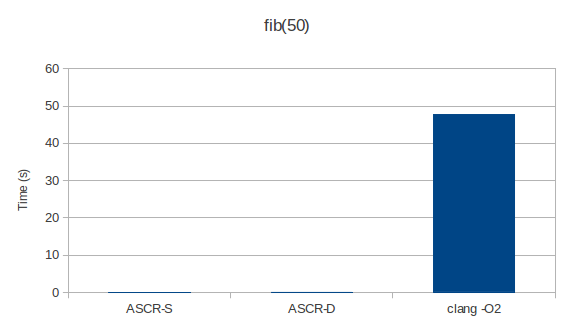
\includegraphics[scale=0.65]{performance.png}
\caption{Performance of \t{fib(50)} using static/dynamic/no ASCR.
(Lower is better.)}
\label{fig:performance}
% ASCR-S: .001
% ASCR-D: .022
% clang -O2: 47.05
\end{figure*}

\begin{figure*}[!ht]
\centering
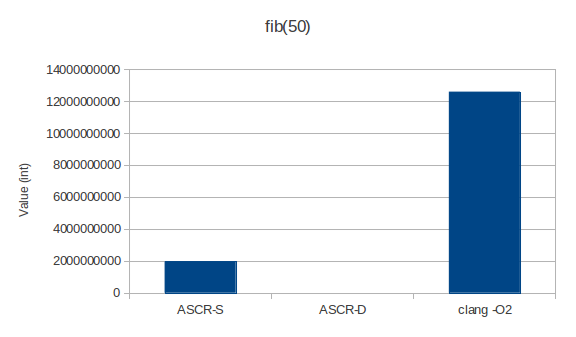
\includegraphics[scale=0.65]{value.png}
\caption{Value of \t{fib(50)} using static/dynamic/no ASCR.
(Lower is better.)}
\label{fig:value}
% ASCR-S: 1957747793
% ASCR-D: 0
% clang -O2: 12586269025
\end{figure*}

\section{Conclusion}

We have shown that address space content randomization is a powerful exploit
mitigation technique which can be applied to programs at compile time without
additional runtime support. ASCR is able to defeat a large class of exploits
which use replay attacks on memory, i.e., by relying on any memory cells to
contain non-random information.

We hope to generalize our current work by also randomizing code in memory,
instead of limiting ourselves to data. This would entirely remove the need for
ASLR, by rendering code pointers---and indeed, code---useless in all situations.
The author is confident that full ASCR, as described above, would in fact
successfully defeat all software exploits.

We believe that the increased effort needed to develop applications which
exhibit desired behavior with ASCR is balanced by the security and performance
afforded by the ASCR regime. In our experiments, when applied in tandem with
traditional compiler optimizations, ASCR results in massively decreased
performance time and runtime values. 

\bibliography{citations}{}
\bibliographystyle{acm}

\end{document}

